\chapter{Introduction to computational linguistics and natural language processing}

\textbf{Computational linguistics (CL)} is a branch of linguistics that focuses on the theoretical understanding of language through computational models. In contrast, \textbf{natural language processing (NLP)} is an interdisciplinary field within artificial intelligence (AI) that aims to use computational models to process and generate language efficiently. NLP intersects with machine learning, statistics, and data science. While NLP is not primarily focused on linguistics, many of its approaches and tasks draw on linguistic theories to address the complexities of natural language. NLP cover a wide range of tasks, including part-of-speech tagging, named entity recognition, machine translation, speech recognition, and text summarization.

\textbf{CL}:
\begin{itemize}
    \item Focuses on modeling human language using computational methods;
    \item Emphasizes theoretical understanding of language;
    \item Grounded in linguistic principles and theories;
    \item Examples include parsing syntactic structures and modeling phonetics.
\end{itemize}

\textbf{NLP}:
\begin{itemize}
    \item Focuses on designing algorithms and systems to process natural language data;
    \item Driven by engineering and computational efficiency;
    \item Examples include machine translation, sentiment analysis, and chatbots.
\end{itemize}

While both share methods and tools such as syntax and semantics modeling or statistical and ML techniques.


\section{Text Preprocessing}

Texts come from diverse sources, languages, formats, scripts, and character encoding standards. A common preliminary step in preparing text for any NLP-related task is \textbf{preprocessing} it to make it suitable for the specific application. Typical preprocessing tasks include removing formatting, converting character encodings, and tokenizing. Additional steps often involve normalizing text, standardizing punctuation, and similar operations. 
A helpful introduction to these strategies and their implications for various NLP tasks can be found in the article \textit{Comparison of text preprocessing methods} \cite{chai2023comparison}. It focuses on tokenization at the word level. However, most neural-network-based approaches rely on subword-level tokenization, which involves splitting words into fragments ranging from single characters to character groups. Some popular subword-level tokenization techniques include byte-pair encoding (BPE), unigram, and SentencePiece.

A concise and intuitive explanation of these methods can be found in the \href{https://huggingface.co/docs/transformers/main/tokenizer_summary}{Tokenizers} section of the HuggingFace Transformers tutorial. Moreover, the \href{https://tiktokenizer.vercel.app/}{Tiktokenizer} is a tool that simulates the tokenization process of several well-known generative neural models. Select a model from the dropdown menu in the upper-right corner and input a short text to see an example of subword tokenization.

\subsection{Format Cleaning}

Raw text data usually contains different formatting elements, such as HTML tags and scripts, metadata and layout information from PDFs, or format marks from Markdown files. In most cases, data related to format adds noise to the text to be processed and should be removed. 

There are different techniques for removing formatting:
\begin{itemize}
    \item \textbf{Regular Expressions (Regex)}: Use patterns to identify and remove unwanted elements, like HTML tags (\plaintt{<.*?>});
    \item \textbf{Libraries and Tools} (usually in Python): \plaintt{BeautifulSoup} for parsing and cleaning HTML or \plaintt{PyPDF2} for extracting text from PDFs;
    \item \textbf{OCR Tools}: For scanned documents, Optical Character Recognition (OCR) tools like \plaintt{Tesseract} can extract text while ignoring formatting.
\end{itemize}

\subsection{Tokenization}

Tokenization decomposes each text string into a sequence of words (technically \textbf{tokens}), which can represent sentences, words, characters or sub-words. 

\paragraph{Sentence Tokenization} This is the process of splitting a text into sentences, using most of the time \textbf{punctuation} marks as delimiters (e.g., periods, exclamation points, question marks). However, this can be challenging due to abbreviations, decimal points, and other punctuation uses that do not indicate sentence boundaries (remember also that not every language use punctuation, see Thai for example). Libraries like \plaintt{NLTK} and \plaintt{spaCy} provide pre-trained models for effective sentence tokenization.

\paragraph{Word Tokenization} This involves splitting a text into words using \textbf{whitespaces}, \textbf{Regex} or \textbf{tailored tokenizers} that can handle specific languages or domains. Challenges include dealing with contractions (e.g., "don't" to "do" and "not"), hyphenated words, and special characters. Again, libraries like \plaintt{NLTK}, \plaintt{spaCy}, and \plaintt{HuggingFace Tokenizers} offer robust word tokenization tools.

\paragraph{Character Tokenization} This method breaks down text into individual characters. It is particularly useful for languages with complex morphology or when dealing with noisy text data, such as social media posts. Character tokenization can also be beneficial in certain NLP tasks like language modeling and text generation. However, it is almost never used alone in modern NLP applications.

\paragraph{Sub-word Tokenization} This technique has become popular in neural-based NLP models, since it addresses issues with rare words and OOV words. Moreover, it is efficient for \textbf{morphologically rich languages} and mantains a balance between word and character tokenization. For this task, different algorithms have been developed, such as \textbf{Byte-Pair Encoding (BPE)}, \textbf{Unigram},\textbf{WordPiece} and \textbf{SentencePiece}. These methods break down words into smaller units based on their frequency in the training corpus, allowing models to handle a wider variety of words and forms. For more details, refer to the \href{https://huggingface.co/docs/tokenizers/index}{HuggingFace Tokenizers documentation}.

\subsection{Text Normalization}

This process aims at converting text into a standard form, reducing variablility in the text while preserving meaning. It also prepares text for consistent and effective processing in NLP tasks. 
Examples include converting text to lowercase, removing punctuation, expanding contractions (e.g., "don't" to "do not"), correcting spelling errors, and standardizing formats for dates, numbers, and abbreviations.

However, modern text is usually encoded with \textbf{Unicode} standards, supporting a wide variety of scipts. This leads to data sparsity at character level. 

Finally, text normalization varies depending on the specific NLP task and language. For instance, in sentiment analysis, preserving certain punctuation (like exclamation marks) may be important, while in machine translation, maintaining the original casing and punctuation is crucial for accuracy. More examples include:
\begin{itemize}
    \item \textbf{Case-sensitive tasks}: Named Entity Recognition (NER), where capitalization can indicate proper nouns;
    \item \textbf{Removing Punctuation}: Useful in BoW models, but not always suitable for tasks like sentiment analysis;
    \item \textbf{Removing redundant text}: Removing duplicates sentences or paragraphs in a corpus is useful when training language models.
\end{itemize}

\subsection{Identifying Stopwords}

Stopwords are common words that carry little meaningful information and are often removed during text preprocessing to reduce noise and improve model performance. Examples include "the", "is", "in", "and", etc. However, the decision to remove stopwords depends on the specific NLP task. For instance, in sentiment analysis, words like "not" can significantly alter the meaning of a sentence and should be retained. They can be detected in different ways, like using a \textbf{predefined stopwords list} (e.g., from \plaintt{NLTK} or \plaintt{spaCy}), by analyzing \textbf{word frequency} in the corpus to identify common words that may not contribute significantly to the task at hand or with \textbf{POS tagging} to identify function words that are typically considered stopwords.

\begin{observationblock}[Zipfian distribution of vocaboulary]
    When the words in a corpus are ranked decreasingly they follow a \textbf{zipfian distribution} in which 
    \[
    freq(r) \propto \frac{1}{r}
    \]
    In other words, a few words in most languages have a very high frequency and most of the words in a language have a very low frequency. This implies that removing stopwords can significantly reduce the vocabulary size without losing much information.
\end{observationblock}

The implications of removing stopwords should be carefully considered based on the specific NLP task and the characteristics of the dataset being used:
\begin{itemize}
    \item \textbf{Focus on meaningful terms}: Removing stopwords can help models focus on more meaningful terms that contribute to the overall context and meaning of the text;
    \item \textbf{Risk of losing context}: In some cases, stopwords can provide important context or nuance to the text. For example, in sentiment analysis, words like "not" can significantly alter the meaning of a sentence;
    \item \textbf{Task-specific considerations}: Some tasks like sentiment analysis may benefit from retaining stopwords.
\end{itemize}

\section{Morphological Parsing}

\textbf{Computational morphology} refers to the design of software that analyzes or generates words not as atomic, indivisible units, but as the intricately structure objects linguistics have long recognized them to be. \textbf{Morphology} is the study of the stucture of words and the rules for word formation in a language. It focuses on the internal structure of words, including \textit{morphemes}, which are the smallest meaningful units of language. In morphological parsing, we break down words into:
\begin{itemize}
    \item \textbf{Lemmas}: Base forms of words (e.g., "running" to "run");
    \item \textbf{Morphemes}: Smallest units of meaning (e.g., "unhappiness" to "un-", "happy", "-ness").
\end{itemize}

This is essential for understanding word formation, meaning and grammatical roles. 

In NLP, morphological parsing is used to simplify texts, extracting information relevant to understand meaning, generating morphologically-correct text and supporting language learners. For low-resource languages, valuable morphological resources are typically small or non-existent \cite{wiemerslage2022morphological}. For richly inflected languages, morphological parsing is crucial to handle the complexity of word forms and their grammatical relationships. The canonical form of a word is called the \textit{lemma}, and the set of all surface forms of it is called the \textit{paradigm}. To help having annotated morphological data with a universal tagset, the \textbf{UniMorph} project has been created \cite{kirov2018unimorph}. It provides a large-scale, multilingual database of morphological paradigms and annotations for over 100 languages, where each inflected form is associated with a lemma, that typically carries its underlying lexical meaning and a bundle of morphological features (e.g., tense, number, case). The database is organized in triplets of the form (lemma, inflected form, morphological features).

\begin{table}[H]
    \centering
    \begin{tabular}{|c|c|c|}
        \hline
        \textbf{Lemma} & \textbf{Inflected Form} & \textbf{Morphological Features} \\
        \hline
        run & running & V;PRS;PROG \\
        run & ran & V;PST \\
        child & children & N;PL \\
        happy & happier & ADJ;COMP \\
        \hline
    \end{tabular}
    \caption{Example entries from the UniMorph database.}
    \label{tab:unimorph_example}
\end{table}

Whereas UniMorph contains type-level annotations, the \textbf{Universal Dependencies (UD)} project provides token-level annotations for sentences in many languages, including morphological features, syntactic dependencies, and part-of-speech tags. UD treebanks are widely used for training and evaluating NLP models on various tasks, including morphological analysis. The structure is useful for morphological tagging at the sentence level, where each word in a sentence is annotated with its morphological features.

\begin{table}[H]
    \centering
    \begin{tabular}{|c|c|c|c|}
        \hline
        \textbf{Word} & \textbf{Lemma} & \textbf{POS Tag} & \textbf{Morphological Features} \\
        \hline
        running & run & VERB & Tense=Pres;Aspect=Prog \\
        ran & run & VERB & Tense=Past \\
        children & child & NOUN & Number=Plur \\
        happier & happy & ADJ & Degree=Comp \\
        \hline
    \end{tabular}
    \caption{Example entries from a Universal Dependencies treebank.}
    \label{tab:ud_example}
\end{table}

In the simplest setting, we simply wish to obtain a detailed morphological summary of a given word. For example, take the word \textit{puppies} in English. A morphological parser should be able to identify that this word is the plural form of the noun \textit{puppy}. Such a task is called \textbf{morphological tagging} and is very useful and valuable for "downstream" tasks, such as \textbf{parsing} \cite{aronoff2022morphology}, recovering the syntactic structure of a sentence. This morhological summary might also include the word \textbf{segmentation}, which might break the word down into its morphemes: \textit{puppy} + \textit{-ies}. This suggests a more sophisticated alternative to stemming: \textbf{lemmatization}, or replacing inflected words with their lemmas. The inverse problem, \textbf{morphological generation}, is a key part on many generative systems.

Nowadays, \textbf{data-driven} methods are the most successful approaches to morphological parsing. These methods typically involve training machine learning models on annotated corpora, such as those provided by the UniMorph and Universal Dependencies projects. In this notes I will focus only on this approach, while the \textbf{knowledge-based} approaches can be found in \cite{aronoff2022morphology}. 

\subsection{Morphological Tagging}

Morphological tagging is a sequence-labeling task similar to part-of-speech tagging. It considers words in context, assigning each word a set of morphological features based on its role in the sentence. For instance, in the sentence "The cats are playing", the word "cats" would be tagged as a noun with plural number. Taggers are important building blocks for many other natural language processing tasks. PoS and morphological tags are used for different "downstream" processing tasks, such as named entity recognition, syntactic parsing, and machine translation. Accurate morphological tagging can improve the performance of these tasks by providing additional linguistic information about the words in a sentence. 

Tagging is a structured prediction problem, that requires us to simultaneously make a series of interdependent decisions to obtain the best overall prediction. One method to address this problem is the \textbf{Hidden Markov Model} (HMM), which tells a simple "story" about how data are produced. It imagines that each tag is generated by the previous tag, and each word is then generated by its tag. 

\begin{figure}[H]
    \centering
    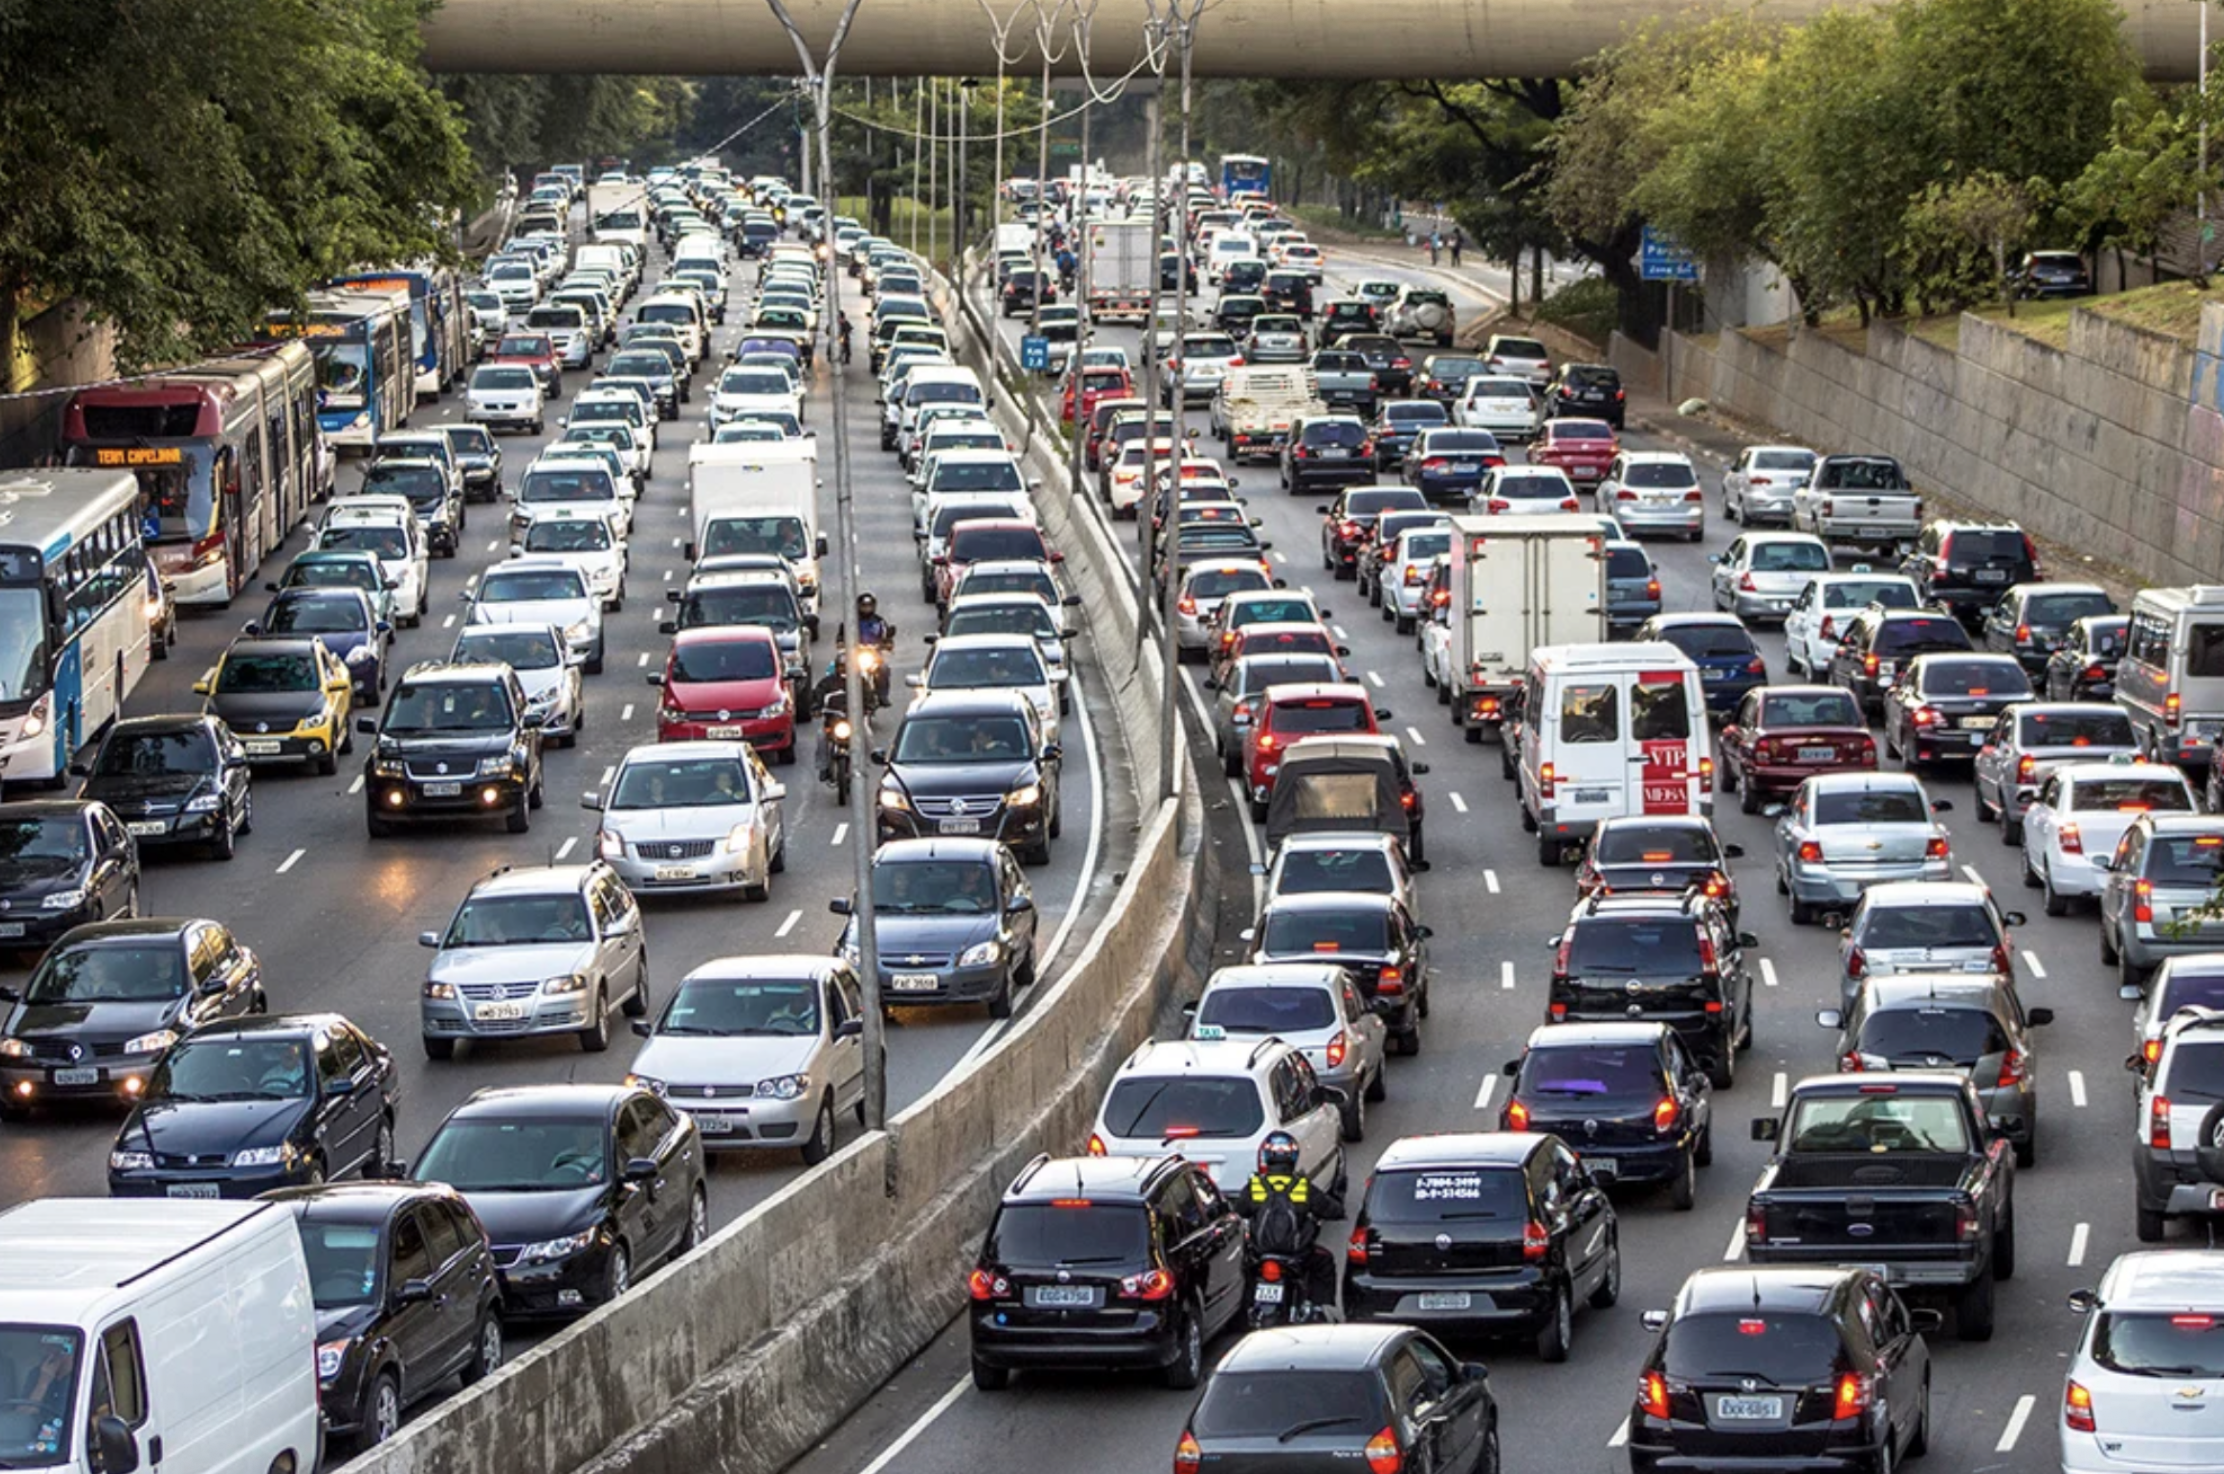
\includegraphics[width=0.7\textwidth]{assets/ch1/1.png}
    \caption{Graphical representation of a Hidden Markov Model for morphological tagging. Each circle represents a hidden state (morphological tag), and each square represents an observed word. Arrows indicate dependencies between states and observations.}
    \label{fig:hmm_morphological_tagging}
\end{figure}

Without going into much details, which you can find in \cite{aronoff2022morphology}, here the Viterbi algorithm can be used to efficiently find the most probable sequence of tags for a given sequence of words. More advanced models, such as Conditional Random Fields (CRFs) and neural network-based approaches (e.g., LSTMs, Transformers), have also been applied to morphological tagging with great success.

\subsection{Morphological Segmentation}

With segmentation, the goal is to split words into their smallest meaning-bearing units: \textbf{morphemes}. There are two types of segmentation:
\begin{itemize}
    \item \textbf{Surface Segmentation}: Splits a word into morphemes in a way such that the concatenation of all parts exactly results in the original word. For example, the word "unhappiness" can be surface-segmented into "un-", "happy", and "-ness". (Note that this is not necessarily meaningful for all languages);
    \item \textbf{Canonical Segmentation}: It is more complex as it aims to split a word into morphemes and to undo the orthographic changes which have occurred during word formation. As a result, each word is segmented into its \textit{canonical} morphemes. For example, the word "running" would be canonically segmented into "run" and "-ing", restoring the base form of the verb.
\end{itemize}

\subsection{Lemmatization, Inflection, Reinflection}
Inflection and reinflection are concerned with generating inflected forms of a lemma. The former generates a word from a given lemma and a set of morphological features, while the latter generates a new inflected form from an existing inflected form and a target set of morphological features. For example, given the lemma "run" and the features "3rd person singular present", an inflection system would generate "runs". Given the inflected form "running" and the target features "past tense", a reinflection system would generate "ran". \textbf{Lemmatization} is the process of reducing an inflected word to its base or dictionary form, known as the lemma. For example, the words "running", "ran", and "runs" would all be lemmatized to "run". It is essentially a special case of the reinflextion and a sort of tagging.Lemmatization is important for various NLP tasks, such as information retrieval and text analysis, as it helps to group together different forms of a word.

Most commonly, these operation refer to type-level tasks. The input consists of an input form together with the target morphosyntactic description (MSD). 

\[
\text{mutated V;3;SG;PRS} \to \text{mutates}
\]

The token-level version of the task is often referred to as lemmatization or inflextion \textit{in context}, meaning that the system has access to the sentential context in which the word appears. This is particularly useful for languages with high levels of homography, where the same surface form can correspond to different lemmas or morphological analyses depending on the context.

\[
\text{mutate - The virus [MASK]} \to \text{mutates}
\]

A drawback of this formulation is that typically many different inflected forms are possible with the same context. To overcome this problem, some approaches model the task as a sequence-to-sequence problem, where the input is the entire sentence with the target word marked, and the output is the inflected form of the target word. This allows the model to learn to generate the correct inflected form based on the context provided by the surrounding words.

\section{Syntactic Parsing}

Syntactic parsing is aimed at determining the structure of a sentence and provides representations that help understand relationships between words. Two main approaches exist: \textbf{constituency parsing} and \textbf{dependency parsing}.

\paragraph{Depencency Structure} Represents syntax as directed relationships between words, capturing dependencies directly. Each word is linked to its dependents, forming a tree structure where the root is typically the main verb. This approach is particularly useful for languages with flexible word order, as it focuses on the relationships between words rather than their positions in the sentence. Take for example sentence "The cat sat on the mat". The dependency structure would identify "sat" as the root verb, with "cat" as its subject and "on the mat" as a prepositional phrase modifying the verb. Below is an illustration of the dependency parse tree for this sentence.

\begin{center}
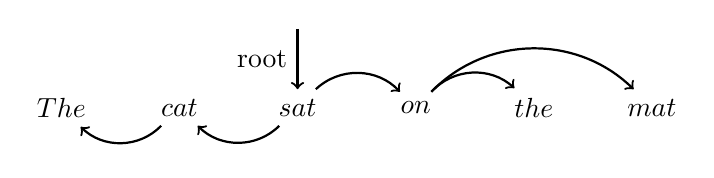
\begin{tikzpicture}[
    roundnode/.style={circle, draw=black, minimum size=1cm},
    directed/.style={->, thick}
]

    % Nodes
    \node (the) at (-3,0) {$The$};
    \node (cat) at (-1.5,0) {$cat$};
    \node (sat) at (0,0) {$sat$};
    \node (on) at (1.5,0) {$on$};
    \node (the2) at (3,0) {$the$};
    \node (mat) at (4.5,0) {$mat$};
    

    % Curve Arrows
    \draw[directed] (sat) to[bend left=45] (cat);
    \draw[directed] (sat) to[bend left=45] (on);
    \draw[directed] (on) to[bend left=45] (the2);
    \draw[directed] (on) to[bend left=45] (mat);
    \draw[directed] (cat) to[bend left=45] (the);

    % Arrow above root (sat) with written "root"
    \draw[directed] (0,1) -- (sat) node[midway, left] {root};
\end{tikzpicture}
\end{center}

Dependency parsing means predicting linguistic structure from input sentences by establishing relationships between "head" words and words which modify those heads. Dependency parsers can be built using various approaches, including rule-based methods, statistical models, and neural network-based techniques. Modern dependency parsers often leverage deep learning architectures, such as BiLSTMs or Transformers, to capture complex syntactic patterns in text. There are two main approaches:
\begin{itemize}
    \item \textit{Transition-based models}: These models build the dependency tree incrementally by making a series of decisions (transitions) based on the current state of the parse. They are typically faster and more efficient, making them suitable for real-time applications. They can easily condition on infinite context, but use greedy search algorithms that can cause short-term mistakes (see \href{https://en.wikipedia.org/wiki/Shift-reduce_parser}{Shift-reduce parsing} for more details);
    \item \textit{Graph-based models}: These models calculate probabilities for each edge/constituent and perform dynamic programming to find the highest-scoring tree. They tend to be more accurate but computationally intensive, making them less suitable for real-time applications. They consider global context and optimize the entire tree structure, but can be slower and require more computational resources (see \href{https://web.stanford.edu/~jurafsky/slp3/old_oct19/15.pdf}{Jurafsky \& Martin, Speech and Language Processing} for more details).
\end{itemize}

\paragraph{Phrase Structure} Represents syntax as nested phrases and is also known as constituency parsing. It breaks down sentences into hierarchical structures of phrases, such as noun phrases (NP) and verb phrases (VP). Each phrase can contain other phrases or words, forming a tree structure that reflects the grammatical organization of the sentence. For the same sentence "The cat sat on the mat", the phrase structure would identify "The cat" as a noun phrase (NP) and "sat on the mat" as a verb phrase (VP). Below is an illustration of the phrase structure parse tree for this sentence.

\begin{center}
\begin{tikzpicture}[level distance=1.5cm,
  level 1/.style={sibling distance=4cm},
  level 2/.style={sibling distance=2cm},
  edge from parent/.style={draw, -latex}]
  \node {S}
    child { node {NP}
      child { node {Det}
        child { node {The} } }
      child { node {N}
        child { node {cat} } } }
    child { node {VP}
      child { node {V}
        child { node {sat} } }
      child { node {PP}
        child { node {P}
          child { node {on} } }
        child { node {NP}
          child { node {Det}
            child { node {the} } }
          child { node {N}
            child { node {mat} } } } } };
\end{tikzpicture}
\end{center}

Dependency parsing is often preferred for its simplicity and direct representation of word relationships, while phrase structure parsing provides a more detailed hierarchical view of sentence structure. The choice between the two approaches depends on the specific NLP task and the linguistic characteristics of the language being analyzed, even if usually the former is easier to apply to languages with different word orders. They help NLP tasks in different ways:
\begin{itemize}
    \item Splitting text into meaningful fragments;
    \item Disambiguating word meanings based on context;
    \item Knowledge-enhanced models (summarization, translation, etc.);
    \item Helping identifying named entities.
\end{itemize}

The project \textbf{Universal Dependencies (UD)} provides a standardized framework for dependency parsing across multiple languages, facilitating cross-linguistic research and applications. UD treebanks are widely used for training and evaluating dependency parsers, making them a valuable resource in the NLP community. Moreover, tools like the \href{https://stanfordnlp.github.io/stanza/}{Stanza} library or SciPy provide pre-trained models for efficient dependency parsing.

\section{Semantic Representation of Text}

\begin{definitionblock}[Semantic compositionality principle]
    The meaning of a complex expression (a \textbf{sentence}) is determined by the meanings of its constituent parts (\textbf{words}) and the way they are combined (\textbf{syntax}).
\end{definitionblock}

A \textbf{lexeme} is a unit of meaning in language, independent of inflectional forms. An example is the lexeme "run", which includes forms like "runs", "running", and "ran". Lexemes are crucial for understanding semantics, as they represent the core meaning of words. The \textbf{word sense}, instead, is the specific meaning of a word in a given context, which can vary based on usage. For example, the word "bank" can refer to a financial institution or the side of a river, depending on the context. Understanding word senses is essential for tasks like word sense disambiguation, where the goal is to determine the correct meaning of a word based on its context.

Words are related by their meaning:
\begin{itemize}
    \item \textbf{Synonymy}: Words with similar meanings (e.g., "big" and "large");
    \item \textbf{Antonymy}: Words with opposite meanings (e.g., "hot" and "cold");
    \item \textbf{Similarity}: Words that are related in meaning but not identical (e.g., "car" and "vehicle");
    \item \textbf{Relatedness}: Words belong to the same \textit{semantic field} (e.g., "doctor" and "hospital").
    \item \textbf{Connotation}: The emotional or cultural associations of a word (e.g., "home" connotes warmth and safety).
\end{itemize}

\textbf{Vector Semantics} is a method of representing word meanings using vectors in a high-dimensional space. Words are represented as points in this space, where the distance between them reflects the semantic similarity of words and words appearing in similar contexts are closer in the vector space. 

There are three main approaches to vector semantics:
\begin{itemize}
    \item \textbf{Bag of Words (BoW)}: Represents documents as a vector of word counts, ignoring grammar, word order and context. Given a corpus (e.g. "The cat sat on the mat."), we represent each document as a vector of word counts (the length of the vector is equal to the size of the vocaboulary, determined through tokenization). In this case, the BoW representation would be [1, 1, 1, 1, 1, 1] for the words ["The", "cat", "sat", "on", "the", "mat"] respectively. This creates a sparse and high-dimensional vector space, which can be computationally expensive to work with;
    \item \textbf{TF-IDF}: Weights words by their importance in the document and corpus, reducing the impact of frequent but uninformative words (e.g. "the"). The first step is to define the \textbf{term frequency (TF)}:
    \[
    \text{TF} = \frac{\text{Number of occurrences of the term in the document}}{\text{Total terms in the document}}
    \]
    Then, we define the \textbf{inverse document frequency (IDF)}:
    \[
    \text{IDF} = \log{\frac{\text{Total number of documents}}{\text{Number of documents containing the term}}}
    \]
    Finally, the \textbf{TF-IDF} score is computed as:
    \[
    \text{TF-IDF} = \text{TF} \times \text{IDF}
    \]
    It is important to take into consideration that TF-IDF may give low scores to semantically important words, and produces, as BoW, sparse and high-dimensional vectors;
    \item \textbf{Embeddings}: Dense vector representations of text in a continuous vector space, they capture the semantic and syntactic relationships between words. Unlike BoW or TF-IDF, embeddings are \textbf{dense} (low-dimensional) and are learned automatically from data rather than being based on simple counting or weighting. Different models and strategies exist to generate embeddings, such as \textbf{Word2Vec}, \textbf{GloVe}, and \textbf{FastText}. More recently, contextual embeddings from models like \textbf{BERT} and \textbf{GPT} have become popular, as they capture the meaning of words in context, allowing for more nuanced representations.
    
    \textbf{Neural Networks} are used to learn embeddings by training on large corpora of text. The networks learn to predict words based on their context (or vice versa), adjusting the vector representations of words to minimize prediction errors. This process results in embeddings that capture semantic relationships, such as synonyms being close together in the vector space. For a recall on neural networks, refer to \cite{jurafskyspeech}.

    To compare two vector representations, a measure of \textbf{distance} or \textbf{similarity} has to be computed, usually with the Euclidean Distance (straight-line distance between vectors) or with the Cosine Similarity (cosine angle between bectors in the vector space). 
    \[
    \text{cosine similarity} = \frac{\vec{u}\cdot \vec{v}}{\|\vec{u}\| \|\vec{v}\|}
    \]
\end{itemize}